% Modelo da UFMG -
% Este modelo foi baseado em: modelo-ufpr.tex,v 1.1 2003/06/30 15:05:18 gweber Exp $
% $Id: modelo-ufpr.tex,v 1.1 2003/06/30 15:05:18 gweber Exp $
%   Licence: LPPL (LaTeX Project Public License)
%     You can change this file in the terms of LPPL
%     (http://www.latex-project.org/lppl.html)
% copyright Rogério C. <rogerioc@cesec.ufpr.br>
%
% ****** DEFINIÇÕES INICIAIS ******	
\documentclass[a4paper,12pt, normaltoc, pnumromarab, pagestart=fistchapter, tocpage=plain]{abnt}
% Utilize a opção normalfigtabnum para numerar as figuras e tabelas por capítulo
%\usepackage[alf]{abntcite} chamada de referencia alfabetica
\usepackage[num]{abntcite}
\usepackage[brazil]{babel}
\usepackage[utf8]{inputenc}
\usepackage[T1]{fontenc}
\usepackage{indentfirst}
\usepackage{graphicx}														%Package para figuras
\usepackage{float}
\usepackage{geometry}
\usepackage{url}
\geometry{a4paper,left=3cm,right=2cm,top=3cm,bottom=2cm}

%%
%%	Ainda em teste
%%
%\usepackage[bookmarks=false]{hyperref}					%Package para hyper-referências
%\hypersetup{colorlinks,
%							citecolor = black,
%							filecolor = black,
%							linkcolor = black,
%							urlcolor  = blue,
%						pdfnewwindow}
%
% O problema ocorre quando há referências do tipo \cite{} e \citeonline{}
% Há ainda outros problemas -> o figura, antes do número, não altera de cor na lista de figuras.
% O mesmo ocorre na lista de tabelas.
% O sumário aponta para a capa, não para o resumo, lista, apêndices ou anexos correspondentes.
% -> Funciona para capítulos.
%

\makeatletter	%Para que ele entenda o @

% Altera o tamanho das fontes dos capítulos e dos apêndices
\renewcommand{\ABNTchapterfont}{\bfseries}
\renewcommand{\ABNTchaptersize}{\Large}
\renewcommand{\ABNTanapsize}{\Large}

%Altera o espaçamento entre dots
%\renewcommand\@dotsep{2}

%Altera forma de montagem do table of contents
\renewcommand\l@chapter[2]{
  \ifnum \c@tocdepth >\m@ne
    \addpenalty{-\@highpenalty}%
    \vskip 1.0em \@plus\p@
    \setlength\@tempdima{1.5em}%
    \begingroup
      \ifthenelse{\boolean{ABNTpagenumstyle}}
        {\renewcommand{\@pnumwidth}{3.5em}}
        {}
      \parindent \z@ \rightskip \@pnumwidth
      \parfillskip -\@pnumwidth
      \leavevmode \normalsize\ABNTtocchapterfont
      \advance\leftskip\@tempdima
      \hskip -\leftskip
      #1\nobreak\dotfill \nobreak%
      \ifthenelse{\boolean{ABNTpagenumstyle}}
         {%
          \hb@xt@\@pnumwidth{\hss
            \ifthenelse{\not\equal{#2}{}}{{\normalfont p.\thinspace#2}}{}}\par
         }
         {%
          \hb@xt@\@pnumwidth{\hss #2}\par
         }
      \penalty\@highpenalty
    \endgroup
  \fi}

\renewcommand*\l@section{\@dottedtocline{1}{0em}{2.3em}}
\renewcommand*\l@subsection{\@dottedtocline{2}{0em}{3.2em}}
\renewcommand*\l@subsubsection{\@dottedtocline{3}{0em}{4.1em}}

% Cria um comando auxiliar para montagem da lista de figuras
\newcommand{\figfillnum}[1]{%
  {\hspace{1em}\normalfont\dotfill}\nobreak
  \hb@xt@\@pnumwidth{\hfil\normalfont #1}{}\par}

% Cria um comando auxiliar para montagem da lista de tabelas
\newcommand{\tabfillnum}[1]{%
	{\hspace{1em}\normalfont\dotfill}\nobreak
	\hb@xt@\@pnumwidth{\hfil\normalfont #1}{}\par}

% Altera a forma de montagem da lista de figuras
\renewcommand*{\l@figure}[2]{
	\leftskip 3.1em
	\rightskip 1.6em
	\parfillskip -\rightskip
	\parindent 0em
	\@tempdima 2.0em
	\advance\leftskip \@tempdima \null\nobreak\hskip -\leftskip
	{Figura \normalfont #1}\nobreak \figfillnum{#2}}

% Altera a forma de montagem de lista de tabelas
\renewcommand*{\l@table}[2]{
	\leftskip 3.4em
	\rightskip 1.6em
	\parfillskip -\rightskip
	\parindent 0em
	\@tempdima 2.0em
	\advance\leftskip \@tempdima \null\nobreak\hskip -\leftskip
	{Tabela \normalfont #1}\nobreak \tabfillnum{#2}}

% Define os comandos que montam a lista de símbolos
\newcommand{\listadesimbolos}{\pretextualchapter{Lista de Símbolos}\@starttoc{lsb}}
\newcommand{\simbolo}[2]{{\addcontentsline{lsb}{simbolo}{\numberline{#1}{#2}}}#1}
\newcommand{\l@simbolo}[2]{
	\vspace{-0.75cm}
	\leftskip 0em
	\parindent 0em
	\@tempdima 5em
	\advance\leftskip \@tempdima \null\nobreak\hskip -\leftskip
	{\normalfont #1}\hfil\nobreak\par}

% Define o comando que monta a lista de siglas
\newcommand{\listadesiglas}{\pretextualchapter{Lista de Siglas}\@starttoc{lsg}}
\newcommand{\sigla}[2]{{\addcontentsline{lsg}{sigla}{\numberline{#1}{#2}}}#1}
\newcommand{\l@sigla}[2]{
	\vspace{-0.75cm}
	\leftskip 0em
	\parindent 0em
	\@tempdima 5em
	\advance\leftskip \@tempdima \null\nobreak\hskip -\leftskip
	{\normalfont #1}\hfil\nobreak\par}

% Define o tipo de numeração das páginas
\renewcommand{\chaptertitlepagestyle}{plain}

% Altera a posição da numeração de páginas dos elementos pré-textuais
\renewcommand\pretextualchapter{
	\if@openright\cleardoublepage\else\clearpage\fi
	\pagestyle{\chaptertitlepagestyle}
	\global\@topnum\z@
	\@afterindentfalse
	\@schapter}

% Altera a posição da numeração de páginas dos elementos textuais
\renewcommand{\ABNTchaptermark}[1]{
	\ifthenelse{\boolean{ABNTNextOutOfTOC}}
		{\markboth{\ABNTnextmark}{\ABNTnextmark}}
		{\chaptermark{#1}
		\pagestyle{\chaptertitlepagestyle}}}

% Redefine o tipo de numeração das páginas
\renewcommand{\ABNTBeginOfTextualPart}{
	\renewcommand{\chaptertitlepagestyle}{plainheader}
	\renewcommand{\thepage}{\arabic{page}}
%	\setcounter{page}{1}
}

\makeatother

%Altera o tamanho do parágrafo
\setlength{\parindent}{1.5cm}

% ********************************
% ***** Início do Documento ******
% ********************************
\begin{document}

%    Modelo de Projeto de TCC
%
% Centro Federal de Educação Tecnológica de Minas Gerais - CEFET-MG
% Autor: Mariane Raquel
%
% Parte: Capa e Folha de rosto projeto

\titulo{Comparação de algoritmos paralelos de ordenação em MapReduce}

\instituicao{Centro Federal de Educação Tecnológica de Minas Gerais \par 					Departamento de Computação \par
			Curso de Engenharia de Computação}

\autor{Mariane Raquel Silva Gonçalves}

\orientador{Profª. Drª. Cristina Duarte Murta}

\comentario{Projeto apresentado como requisito parcial à aprovação em Trabalho de Conclusão de Curso I do curso de Engenharia de Computação do Centro Federal de Educação Tecnológica de Minas Gerais.}

\local{Belo Horizonte}

\data{2012}

\logo{figuras/logo.pdf}

\capa

\folhaderosto


%% -------------------------------------------------------
%% --------------------- CAPA ----------------------------
%% -------------------------------------------------------
%
%\begin{titlepage}
%
%% Logo e Universidade
%\begin{flushleft} 
%\begin{minipage}{0.25\textwidth}
%
\includegraphics[scale=0.7]{figuras/logo.png} 
%\end{minipage} \hfill
%\begin{minipage}{0.7\textwidth}
%\begin{flushleft} \begin{center} 
%Centro Federal de Educação Tecnológica de Minas Gerais \\ Departamento de Computação \\ Curso de Engenharia de Computação 
%\end{center} \end{flushleft} 
%\end{minipage} 
%\end{flushleft}
%\begin{center}
%% Aluno 
%\vspace{1.5cm} Mariane Raquel Silva Gonçalves
%% Título
%\vspace{5cm} 
%\begin{espacoduplo} 
%\begin{Large} \textbf{ \textsc{Comparação de algoritmos paralelos de ordenação em MapReduce}}  \end{Large} \\
%\end{espacoduplo}
%% Orientador
%\vfill Orientadora: Profª. Drª. Cristina Duarte Murta \\[1cm]
%% Data
%Belo Horizonte \\ 2012 \\
%\end{center}
%\end{titlepage}
%
%
%% -------------------------------------------------------
%% ----------------- FOLHA DE ROSTO ----------------------
%% -------------------------------------------------------
%\instituicao{Centro Federal de Educação Tecnológica de Minas Gerais \\ Departamento de Computação \\ Curso de Engenharia de Computação}
%
%\autor{ Mariane Raquel Silva Gonçalves} 
%
%\titulo{Comparação de algoritmos paralelos de ordenação em MapReduce}
%
%%\tituloformat = sc, bf, Large
%
%\orientador{Profª. Drª. Cristina Duarte Murta} 
%
%%LOGO 
\includegraphics[scale=0.7]{figuras/logo.png}
%
%\comentario{Projeto apresentado como requisito parcial à aprovação em Trabalho de Conclusão de Curso I do curso de Engenharia de Computação do CEFET-MG. }
%
%\folhaderosto
%%\begin{titlepage}
%%
%%% Logo e Universidade
%%\begin{flushleft} 
%%\begin{minipage}{0.25\textwidth}
%%
\includegraphics[scale=0.7]{figuras/logo.png} 
%%\end{minipage}
%%\hfill
%%\begin{minipage}{0.7\textwidth}
%%\begin{flushleft} 
%%\begin{center} Centro Federal de Educação Tecnológica de Minas Gerais \\ Departamento de Computação \\ Engenharia de Computação \end{center}
%%\end{flushleft}
%%\end{minipage}
%%\end{flushleft}
%%
%%\begin{center}
%%% Aluno 
%%\vspace{1.5cm} Mariane Raquel Silva Gonçalves
%%% Título
%%\vspace{5cm} 
%%\begin{espacoduplo}  \begin{Large} \textbf{ \textsc{Comparação de algoritmos paralelos de ordenação em MapReduce}}  \end{Large} \\ \end{espacoduplo}
%%\end{center}
%%
%%% Texto
%%\vfill
%%\begin{flushright}
%%\begin{minipage}{0.5\textwidth}
%%Projeto apresentado como requisito parcial à aprovação em Trabalho de Conclusão de Curso I do curso de Engenharia de Computação do CEFET-MG. 
%%\end{minipage}
%%\end{flushright}
%%\vfill
%%
%%\begin{center}
%%% Orientador
%%Orientadora: Profª. Drª. Cristina Duarte Murta \\[1cm]
%%% Data
%%Belo Horizonte \\ 2012 \\ 
%%\end{center}
%%\end{titlepage}
%


\begin{titlepage}
\begin{center}
Universidade Federal de Minas Gerais \\
Instituto de Ciências Exatas \\
Departamento de Ciências da Computação \\
\end{center}
\vfill
% comentário 
\comentario

\begin{center}
%\hspace{.45\textwidth} % posicionando a minipage
\framebox[.8\textwidth][c]{
\begin{minipage}{.7\textwidth}
\begin{center}
\vspace{1cm}
\textbf{Rastreamento por telefonia móvel utilizando Android} \\
\vspace{2em}
por \par
\vspace{2em}
{Raphael Ottoni Santiago Machado de Faria} \\
\vspace{2em}
Monografia de Projeto Orientado em Computação I \\
\vspace{1em}
\begin{center}
\footnotesize{Apresentado como requisito da disciplina de Projeto Orientado em Computação I do Curso de Bacharelado em Ciência da Computação da UFMG} \\
\end{center}
\vspace{1em}
Prof. Dr. Fernando Magno Quintão Pereira\\
Orientador
\vspace{1cm}
\end{center}
\flushleft
Assinatura do Aluno:\\
\vspace{1cm}
Assinatura do Professor:\\
\vspace{1cm}
\end{minipage}
}

\vfill
Belo Horizonte -- MG \\
2010 / 2º semestre
\end{center}
\end{titlepage}



\begin{folhadeaprovacao} 

% Logo e Universidade
\begin{flushleft} 
\begin{minipage}{0.25\textwidth}

\includegraphics[scale=0.7]{figuras/logo.png} 
\end{minipage}
\hfill
\begin{minipage}{0.7\textwidth}
\begin{flushleft}
\begin{center}
Centro Federal de Educação Tecnológica de Minas Gerais \\
Departamento de Computação \\
Curso de Engenharia de Computação
\end{center}
\end{flushleft}
\end{minipage}
\end{flushleft}

\vfill

%\hspace{.45\textwidth} % posicionando a minipage
\framebox[.8\textwidth][c]{
\begin{minipage}{.7\textwidth}
\begin{center}
\vspace{1cm}
\textbf{\textsc{Comparação de algoritmos paralelos de ordenação em MapReduce}} \\
\vspace{2em} 
Trabalho de Conclusão de Curso I \\ 
\vspace{2em}
\setlength{\ABNTsignthickness}{0.4pt} \setlength{\ABNTsignskip}{1cm}
\hspace*{1cm}
\assinatura{Mariane Raquel Silva Gonçalves \\ Aluna} 
\hspace*{1cm}
\assinatura{Profª. Drª. Cristina Duarte Murta \\ Orientadora}
\vspace{1cm}
\end{center} 
\end{minipage}
}
\vfill
\end{folhadeaprovacao}

%% -------------------------------------------------------
%% --------------------- TESTES ---------------------------
%% -------------------------------------------------------
%%
%%	
%%%Folha de aprovação
%%\begin{folhadeaprovacao}
%%Tese para aprovação na faculdade de adminisotração
%%\assinatura{Prof. Um professor \\ Orientador}
%%\assinatura{Prof. Outro Professor  \\ Universidade Federal do Rio Grande do Sul}
%%\assinatura{Prof. Paulo Caroli \\ Gerente Thoughtworks }
%%\end{folhadeaprovacao}
%



% Dedicatória

%\pretextualchapter{}
%\vspace{8cm}
%\begin{flushright}
%\hfill \textnormal{
%Aos professores, \\
%aos colegas de curso e \\
%aos meus familiares, \\
%dedico este trabalho.}
%\end{flushright}


% Agradecimentos 

%\pretextualchapter{Agradecimentos}
%
%\begin{minipage}{\textwidth}
%    Agradeço aos meus pais, pelo amor incondicional. \\
%    Aos meus professores, pelos conhecimentos adquiridos. \\
%     E finalmente aos colegas de curso pela convivência e trocas de experiências.
%\end{minipage}

%  Epígrafe 

%\pretextualchapter{}
%\vspace{8cm}
%\begin{flushright}
%\textnormal{``Pshaw, my dear fellow, what do the public, the great unobservant public, who could hardly tell a weaver by his tooth or a compositor by his left thumb, care about the finer shades of analysis and deduction!'' \\
%	\bfseries Sherlock Holmes, in ``The Adventure of the Copper Beeches``}
%\end{flushright}



%
% Documento: Dedicatória
%

\begin{dedicatoria}
Espaço reservado para dedicatória.
Inserir seu texto aqui...
\end{dedicatoria}



% Agradecimentos - é so para as pessoas que contribuiram relevantemente
% para a elaboração do trabalho
\pretextualchapter{Agradecimentos}

\begin{minipage}{\textwidth}
    Agradeço aos meus pais, pelo amor incondicional. \\
    Aos meus professores, pelos conhecimentos adquiridos. \\
     E finalmente aos colegas de curso pela convivência e trocas de experiências.
\end{minipage}



%
% Documento: Epígrafe
%

\begin{epigrafe}

\textit{``O fator decisivo para vencer o maior obstáculo é, invariavelmente, ultrapassar o obstáculo anterior.'' (Henry Ford)}

\end{epigrafe}


\sumario

% 1 - Lista de Figuras
\listadefiguras

% 2 - Lista de Tabelas
%\listadetabelas

% 3 - Lista de Siglas
% Forma de uso: \sigla{sigla}{Descrição}
%\listadesiglas


\begin{center}

{\bf Resumo}
\end{center}

Este trabalho apresenta ... escrever um bom resumo ap\'os finalizar a escrita do texto. 


\begin{abstract}
	
    This paper aims to create a scalable and robust  tracking system for the mobile phone network, using \emph{smartphones} with the \emph{Android} operational system.
The ideia is to add a functionality of execution of remote commands to the tracking system, thus creating a wider range of applications and possibilities. An sample of those new 
features would be in the theft case, because with this functionality the cellphone  owner would easily erase his private information such as contacts, messages and data. 

    \par
    \textbf{Keywords}: Android, Pattern: Command, Java, Google App Engine, Cloud Computing, Tracking, mobile network	
\end{abstract}


\chapter{Introdu��o}\label{introducao}

% TEXTO DE MIRELLA M. MORO

\redcomment{(CONTEXTO:)} Ningu�m nasce sabendo, as pessoas nascem sem saber caminhar e  muito menos falar. Tanto caminhar quanto falar requerem ensino e treinamento, num processo de aprendizagem. Igualmente, nenhum estudante entra na Universidade sabendo escrever uma monografia, seja de gradua��o ou p�s. Alguns alunos, por iniciativa pr�pria, buscam literatura espec�fica, como v�rios livros sobre metodologia cient�fica, antes de escrever uma monografia \citep{BoothCW08,GraffB09,TrainaT2009,Turabian07,Wazlawick09,Zobel04}. Por�m, esses s�o poucos. Al�m disso, nesse contexto, cabe ao professor-orientador ``ensinar'' o estudante a escrever a monografia. \redcomment{(PROBLEMA:)} Um problema ainda existe: nem sempre o orientador tem o tempo necess�rio para ensinar cada estudante a escrever. 



\redcomment{(SOLU��O:)} Este documento, que utiliza a classe de \citep{CamaraNeto2011}, visa auxiliar estudantes e professores no momento de escrever a monografia seja de gradua��o ou p�s em Computa��o. V�rias das dicas s�o espec�ficas para a �rea de Computa��o, visto que outras �reas possuem caracter�sticas peculiares de escrita e apresenta��o de ideias.  A finalidade n�o � abordar todas as op��es e exce��es, e sim, prover uma vis�o abrangente para alunos que est�o no est�gio final de gradua��o e p�s-gradua��o. De um modo geral, este documento apresenta uma ``receita de bolo pr�tica'' com dicas sobre estrutura, conte�do e estilo. Espera-se que ao final, o estudante tenha aprendido o b�sico para come�ar a escrever seu trabalho final de curso.

\redcomment{(OUTROS DETALHES:)} Este texto est� organizado da seguinte forma: cada cap�tulo e se��o autoabordam o seu conte�do. Ou seja, o resumo apresenta como o resumo deve ser escrito, a introdu��o como a mesma deve ser organizada e assim por diante.  Por exemplo, considere o seguinte esqueleto (cada item � um cap�tulo): Capa (Autor e T�tulo), Resumo, Introdu��o, Desenvolvimento, Conclus�o e Refer�ncias.  Cada um desses itens � detalhado nos pr�ximos cap�tulos e se��es.


%%%%%%%%%%%%%%%%%%%%%%%%%%%%%%%%%%%
\section{Conte�do da Introdu��o}\label{intro:conteudo}
%%%%%%%%%%%%%%%%%%%%%%%%%%%%%%%%%%%

Ap�s o resumo, � necess�rio escrever a introdu��o da monografia. Em todo o texto, � importante preservar: unidades de apresenta��o claras, organiza��o, precis�o e simplicidade, fluxo natural de ideias e continuidade (toda parte cont�m in�cio, meio e fim). Com isso em mente, a introdu��o � uma vers�o estendida do resumo: tudo o que � mencionado no resumo �  detalhado na introdu��o. As seguintes observa��es se aplicam �\footnote{Este documento tamb�m apresenta algumas regras de portugu�s resumidas para alguns dos casos mais comuns de descuidos. As regras s�o apresentadas em maroon e em rodap�.}\footnote{\portugues{\textbf{Crase}. A crase � a fus�o de duas vogais da mesma natureza. Regra geral: usa-se \textbf{�} diante de palavra do g�nero feminino quando, substituindo-se a feminina por uma masculina, aparecer diante da masculina o \textbf{ao}. Exemplos: se aplicam � introdu��o e ao cap�tulo (com crase pra a palavra feminina); por�m, conhe�o a cidade e o trabalho (sem crase). � proibido crase antes de nomes masculinos, verbos, entre palavras repetidas, pronome de tratamento (senhora, senhorita), pronomes indefinidos (exce��o: outra/s). � facultativo seu uso diante de pronome possessivo (n�o conte � sua m�e = n�o conte a sua m�e) e nomes de pessoas no feminino.
}} introdu��o: 

\begin{itemize}
	\item Uma introdu��o bem escrita � fundamental para nortear o leitor em rela��o ao trabalho detalhado no texto;
	\item Uma monografia N�O � um livro de suspense no qual o  leitor s� descobre o que est� realmente acontecendo no  cap�tulo final;
	\item O leitor deve estar ciente do que acontece desde o in�cio,  desde a introdu��o;
	\item Geralmente, a introdu��o � uma reafirma��o do  conte�do do Resumo. 
\end{itemize}




� importante notar que uma das caracter�sticas mais importantes e dif�ceis de aprender � o \textbf{fluxo de informa��o}. Por exemplo, a Figura \ref{fig:fluxo} considera um artigo que tenha limite de p�ginas (o que n�o � o caso da monografia). Essa figura ilustra que: o t�tulo sempre cont�m uma ou duas palavras-chave (palavras essenciais) que representam o t�pico  ou o conjunto de t�picos do texto; essas palavras-chave s�o especificadas melhor (ou contextualizadas) em uma ou  duas frases do resumo; ent�o a introdu��o estende o resumo, repetindo e especificando ainda mais as ideias apresentadas; a introdu��o tamb�m descreve de maneira geral as principais contribui��es do trabalho bem como os resultados experimentais (ou de valida��o); o texto ent�o decorre sobre os trabalhos relacionados, contribui��es e valida��o da proposta; finalmente, a conclus�o resume, com outras palavras, as principais contribui��es do texto, enfatizando diferen�as, semelhan�as, vantagens e desvantagens. Trazendo esse fluxo para a monografia: o resumo pode conter v�rias linhas para cada palavra central, a introdu��o pode conter mais de um par�grafo para cada uma dessas linhas e assim por diante.

\begin{figure}[tb] % [b] (de bottom) � para colocar a figura ao final da p�gina; [t] (de top)  � para o topo da p�gina
    \centering
    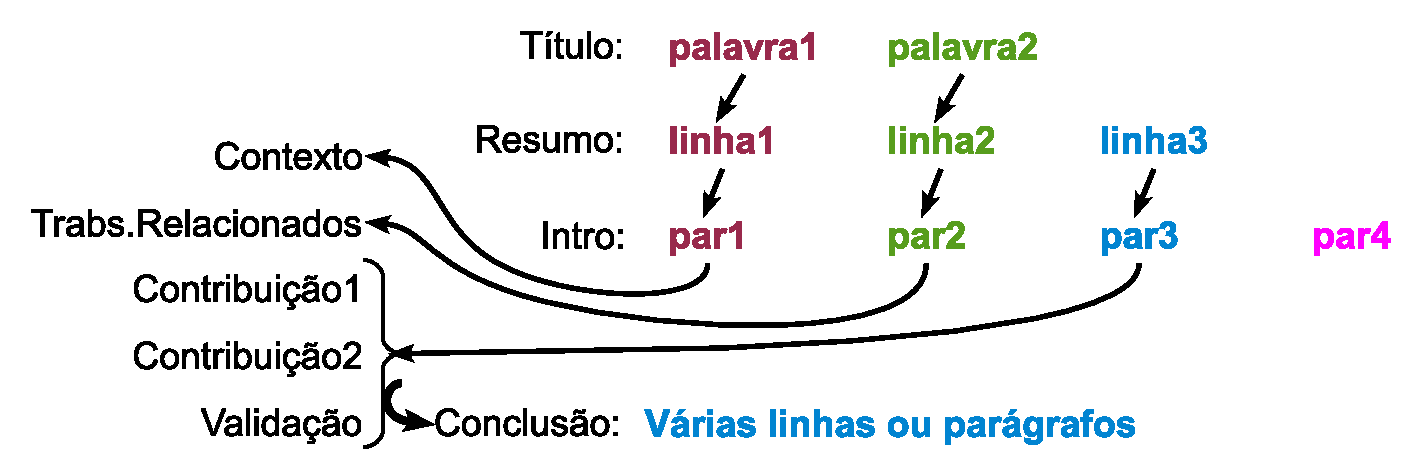
\includegraphics[scale=.6]{img/fluxo} % caso queira mudar o tamanho da figura
    \caption{Fluxo de ideias}
    \label{fig:fluxo}
\end{figure}

A seguir s�o apresentadas duas sugest�es para a introdu��o de trabalhos em Computa��o, a qual deve incluir um ou dois par�grafos para: 

\begin{enumerate}
	\item Identificar a �rea de interesse (palavras do t�tulo), prover o contexto (revis�o b�sica do estado-da-arte), definir o prop�sito do trabalho e/ou hip�tese sendo investigada (exemplos: \textit{O prop�sito deste trabalho � definir...}, \textit{Este trabalho prop�e tr�s m�todos para...}), apresentar a solu��o a ser detalhada (caracter�stica fundamental, t�cnica ou metodologia, vantagens) e a organiza��o do texto;
	\item Identificar o contexto e a motiva��o para o trabalho, especificar o problema em quest�o, discutir trabalhos anteriores relacionados (principalmente as suas limita��es), definir as contribui��es, enfatizar os resultados principais e a organiza��o do texto.
\end{enumerate}

A seguir, cada uma dessas partes � explicada em maiores detalhes.

%%%%%%%%%%%%%%%%%%%%%%%%%%%%%%%%%%%
\section{Introdu��o Passo a Passo}\label{intro:parte}
%%%%%%%%%%%%%%%%%%%%%%%%%%%%%%%%%%%

Independente da sugest�o utilizada, alguns componentes s�o  importantes na introdu��o. Este\footnote{\portugues{\textbf{Este, esse, aquele}. ESTE: perto de quem fala; tempo presente; aquilo que ser� nominado. ESSE: perto de com quem se fala; tempo passado ou futuro; aquilo que j�  foi nominado. AQUELE: longe de quem fala e de com quem se fala; passado vago ou remoto. Ou seja: \textbf{neste} documento, usa-se ESSE para referenciar partes que j� foram especificadas (e.g., Trazendo esse fluxo e ESTE para o que ainda vai se especificar ou para se referenciar ao texto atual (e.g., Este trabalho)}.} documento apresenta cada um  deles individualmente, com exemplos retirados novamente de  artigos cient�ficos (na verdade, artigos cient�ficos podem ser considerados vers�es enxutas da monografia; por isso, utiliz�-los como exemplo faz muito sentido).  

\subsection{Introdu��o: Contexto}

O contexto faz parte da motiva��o do trabalho. Essa parte pode ser tamb�m a evolu��o de um contexto. Por exemplo, considere o in�cio da introdu��o do trabalho \cite{RaghavanVRYS07}.

\begin{Exemplo}
Yesterday's version of distributed computing was a selfcontained, colocated server farm.  
Today, applications are increasingly deployed on third-party resources hosted across
the Internet.  Indeed, the rapid spread of open protocols and standards like Web 2.0 has fueled an explosion of compound services that script together third-party components to deliver a sophisticated service [27, 29]. These specialized services are just the beginning: flagship consumer and enterprise  applications are increasingly being delivered in the softwareas-a-service  model [9]. For example, Google Documents, Groove Office, and Windows Live are early examples  of desktop applications provided in a hosted environment, and  represent the beginning of a much larger trend.
\end{Exemplo}

Nesse primeiro trecho da introdu��o do trabalho, os autores discursam sobre a evolu��o do contexto: computa��o distribu�da. Especificamente, eles falam do ontem e do hoje, enfatizam os componentes do contexto (protocolos, padr�es e servi�os) e finalizam mencionando aplicativos reais que exemplificam o contexto.

\subsection{Introdu��o: Problema}
Uma maneira de evidenciar a contribui��o do trabalho � definir bem o problema a ser resolvido. Nesse caso, pode-se discutir: o problema em quest�o, a defini��o formal do problema  e sua import�ncia, relev�ncia, aplica��es pr�ticas.  Por exemplo, considere a defini��o do problema da introdu��o do trabalho \cite{RaghavanVRYS07}.

\begin{Exemplo}
One of the  key barriers  to moving traditional applications to  the cloud, however, is the loss of cost control [17].  In the cloudbased services model, cost recovery is typically accomplished  through metered pricing. Indeed, Amazon's EC2 charges  incrementally per gigabyte of traffic consumed [3] [...]\footnote{Note que [...] denota que o texto original cont�m outras partes que foram retiradas para simplifica��o do exemplo. Sugere-se a leitura do texto original para o conte�do completo.} Limiting global resource consumption in a distributed  environment, however, presents a   significant technical  challenge. Ideally, resource providers would not require  services to specify the resource demands of each distributed  component a priori; such fine-grained measurement and  modeling can be challenging for rapidly evolving services.  Instead, they should provide a fixed price for an aggregate,  global usage, and allow services to consume resources  dynamically across various locations, subject to the specified  aggregate limit. 
\end{Exemplo}

Nesse trecho seguinte, os autores especializaram o contexto geral (computa��o distribu�da) para o contexto espec�fico da computa��o em nuvens. Al�m de especificar o contexto, os autores tamb�m discutiram os problemas encontrados em torno da perda do controle de custo.

\subsection{Introdu��o: Relacionados}

Outra maneira de evidenciar a contribui��o do trabalho � discutir os trabalhos relacionados (resumidamente) ainda na introdu��o.
Esses trabalhos est�o no mesmo contexto, n�o resolvem o problema ou apresentam apenas solu��es parciais.
Al�m disso, o trabalho atual pode ser a extens�o ou continua��o de um trabalho anterior. Nesse caso, o trabalho original deve ser mencionado na introdu��o.
Pode-se tamb�m agrupar trabalhos similares e detalhar um ou dois. Por exemplo: \textit{Como resposta a tal requisito, alguns trabalhos t�m enfocado 
a quest�o do suporte a vers�es [2,4,9,13,23,27]. Entre esses, 
Golendziner prop�e o Modelo de Vers�es: uma extens�o 
aplic�vel a modelos de dados orientado a objetos ... [9].}

Outra maneira de agrupar os trabalhos relacionados, ainda na introdu��o, � classific�-los. Por exemplo, considere o trecho a seguir retirado de \cite{MoroBT07}.

\begin{Exemplo}
Regarding message content and profile definitions, pub-sub systems have evolved from simple topic-based communication [24,35], to predicate-based systems [10,11], to recently designed XML-aware systems [7,8,9,18,36,37]. Given the adoption~of~XML~as the standard format for data exchange, in this paper we focus on the XML-aware pub-sub systems. In such scenario, messages are encoded as XML documents~and~the~profiles (query subscriptions) are expressed using XML query languages,~such~as~XPath[3].
\end{Exemplo}

\dica{Por uma quest�o de estilo, quando se utilizar refer�ncias num�ricas, uma boa sugest�o � coloc�-las em ordem crescente. Isso facilita o trabalho do leitor de conferir mais de uma refer�ncia ao mesmo tempo.}

Nesse trecho, os autores classificaram os sistemas atuais em tipos de acordo com a evolu��o dos mesmos. Mais adiante na introdu��o, os problemas de tais sistemas foram usados para introduzir a solu��o apresentada no artigo, conforme a seguir.

\begin{Exemplo}
All the previous approaches provide different advantages for various types of queries. However, they all have the same limitation: they do not provide any early pruning feature in their matching algorithm so as to quickly identify (and thus discard) queries that are bound not to match any documents. Considering the increasing volume of incoming message documents and incoming queries, an early pruning technique is essential for saving processing time on the matching process.
\end{Exemplo}

\subsection{Introdu��o: Contribui��es} 
Uma parte \textbf{central} da introdu��o � descrever explicitamente as contribui��es do trabalho. Tal descri��o pode ser simples em um par�grafo, por exemplo: \textit{Considerando o contexto atual, este trabalho prop�e ...}. Ou, pode ser mais trabalhada e delimitada por itens, como em  \cite{RaghavanVRYS07}: \\
 
\begin{Exemplo} 
This paper makes three primary contributions: \\ 
- \textbf{Rate Limiting Cloud-based Services.} We identify a key challenge... \\ 
- \textbf{Distributed Rate Limiter Design.} We present the design ...\\ 
- \textbf{Evaluation and Methodology.} We develop a methodology... 
\end{Exemplo}

Note que nesse artigo, os autores conseguem definir os tr�s pontos principais da contribui��o em poucas palavras. Essa n�o � uma tarefa simples, mas certamente ajuda o leitor a entender melhor as reais contribui��es do artigo e a referenci�-las mais tarde.

Veja que no caso de uma tese de doutorado, o processo � exatamente o mesmo. Por exemplo, veja esta se��o da tese de \cite{Cordeiro2011}.

\begin{Exemplo}
1.3 Main Contributions of this Ph.D. Work \\
\indent With regard to the task of clustering large sets of complex data, an analysis of the
literature (see the upcoming Chapter 3) leads us to come to one main conclusion. In
spite of the several qualities found in the existing works, to the best of our knowledge,
there is no method published in the literature, and well-suited to look for clusters
in sets of complex objects, that has any of the following desirable properties: (i)
linear or quasi-linear complexity -- to scale linearly or quasi-linearly in terms of
memory requirement and execution time with regard to increasing numbers of points
and axes, and; (ii) Terabyte-scale data analysis -- to be able to handle datasets
of Terabyte-scale in feasible time. On the other hand, examples of applications with
Terabytes of high-dimensionality data abound: weather monitoring systems and climate
change models, where we want to record wind speed, temperature, rain, humidity,
pollutants, etc; social networks like Facebook TM, with millions of nodes, and several
attributes per node (gender, age, number of friends, etc); astrophysics data, such as the
SDSS (Sloan Digital Sky Survey), with billions of galaxies and attributes like red-shift,
diameter, spectrum, etc. Therefore, the development of novel algorithms aimed at
overcoming these two aforementioned limitations is nowadays extremely desirable.
This Doctoral dissertation focuses on overcoming both limitations. Specifically, it
presents three novel, fast and scalable data mining algorithms well-suited to analyze large
sets of complex data: \\
~\\
\indent 1. The Method Halite for Correlation Clustering: the algorithm Halite is a fast [...] \\
\indent 2. The Method BoW for Clustering Terabyte-scale Datasets: the method BoW focuses on the problem of [...] \\
\indent 3. The Method QMAS for Labeling and Summarization: the algorithm QMAS uses  [...] \\
~\\
\indent Our algorithms were evaluated on real, very large datasets with up to billions of
complex elements, and they always presented highly accurate results, being at least one
order of magnitude faster than the fastest related works in almost all cases. The real
life data used come from the following applications: automatic breast cancer diagnosis,
satellite imagery analysis, and graph mining on a large web graph crawled by Yahoo! and
also on the graph with all users and their connections from the Twitter social network. In
extreme cases, the work presented in this Doctoral dissertation allowed us to spot in only
two seconds the clusters present in a large set of satellite images, while the related works
took two days to perform the same task, achieving similar accuracy. Such results indicate
that our algorithms allow the development of real time applications that, potentially,
could not be developed without this Ph.D. work, like a software to aid on the 
fly the diagnosis process in a worldwide Healthcare Information System, or a system to look for
deforestation within the Amazon Rainforest in real time.
\end{Exemplo}


Essa se��o da tese de doutorado � absolutamente perfeita: relembra qual � o principal problema do estado da arte, introduz as tr�s principais contribui��es do trabalho e finaliza com um resumo dos principais resultados obtidos com a avalia��o experimental. Uma outra sugest�o � colocar a hip�tese e os objetivos em se��es distintas, conforme utilizado em \cite{Odon2011}.

\begin{Exemplo}
1.2 Hyphothesis \\
\indent In this work, we explore the hypothesis that it is possible to use Wikipedia as an alternative source of geographic evidence to help dealing with the problem of automatically associating places to texts.\\
~ \\
1.3 Objectives
\\
\indent In order to verify the hypothesis, we pursue two ideas in this dissertation. First, we formulate [...] Second, we use a topic indexing technique [...]
\end{Exemplo}


Independente da sugest�o adotada, est� claro que as contribui��es devem ser adequadamente enfatizadas desde a introdu��o do trabalho.

\subsection{Introdu��o: Organiza��o}
Este par�grafo geralmente encerra a introdu��o e � opcional. Outro exemplo � a organiza��o deste documento. 
O Cap�tulo \ref{desenvolvimento} discute as partes centrais do desenvolvimento do texto.
O Cap�tulo \ref{outros} introduz outros pontos importantes como figuras e tabelas, divis�o do texto, entre outros. 
O Cap�tulo \ref{conclusao} conclui este documento com a discuss�o sobre o que � a conclus�o de um texto. 
Finalmente, s�o inclu�dos dois ap�ndices e dois anexos na seguinte ordem: ap�ndice com a defini��o de \textit{ap�ndice} e \textit{anexo} de acordo com a ABNT; ap�ndice de exemplo para mostrar a sequ�ncia da numera��o; anexo livre; e um segundo anexo \textbf{super importante} com um tutorial de LaTex para principiantes (leitura obrigat�ria para quem nunca usou LaTex e n�o tem medo de tentar software livre).


%Por exemplo: 
%\textit{O restante deste trabalho est� organizado da seguinte  maneira. A se��o 2 apresenta alguns conceitos b�sicos e  discute trabalhos relacionados. A se��o 3 detalha o modelo  proposto. A se��o 4 apresenta um estudo comparativo atrav�s  de experimentos, enquanto a se��o 5 conclui o trabalho.}



\chapter{REFERENCIAL TEÓRICO}
\emph{Cloud Computing} é um paradigma relativamente novo, que se refere tanto para aplicações
providas como serviço pela internet quanto para o \emph{hardware} e os sistemas de softwares usados
nos \emph{datacenters} que os provêm. Estes serviços providos são reconhecidos como \emph{Software
as a Service} e a parte de \emph{datacenters} e \emph{softwares} é definida como uma  
\emph{cloud}\cite{clouds}. Pretende-se aproveitar de todas  as vantagens providas por este paradigma, destacando entre elas a
escalabilidade, o  fácil acesso, o baixo custo e a fácil manutenção.\\

Entre as \emph{public clouds} disponíveis ( Amazon EC2, Google Appengine e Windows Azure ),
escolheu-se a \emph{Google Appengine}\footnote{\url{http://code.google.com/appengine/}} por fornecer um ambiente de desenvolvimento gratuito e por sua
facilidade de integração tanto com os outros serviços google como para o próprio \emph{Android}, o
que é vital para o projeto proposto, uma vez que o \emph{google maps} é essencial para a ideia de
rastreamento.\\

Para o desenvolvimento do aplicativo \emph{Android} será utilizado o ambiente de desenvolvimento
\emph{Android SDK}\footnote{\url{http://developer.android.com/sdk/index.html}} fornecido pelo
\emph{Android Open Source Project}\footnote{{http://developer.android.com/index.html}}. \\

Durante o desenvolvimento do serviço na \emph{Cloud Computing} e do aplicativo \emph{Android}
pretende-se aplicar fundamentos da metodologia de desenvolvimento de software conhecida como
\emph{scrum}, que é baseada em conceitos da metodologia \emph{agil}, juntamente com a ideia de desenvolvimento baseado em \emph{test driven design},
em que os testes de unidade são criados primeiro, antes mesmo do próprio código. Espera-se que com a adoção destas práticas o
processo de desenvolvimento seja mais organizado, mais voltado para \emph{refactoring}\footnote{Processo de re-escrita do código com o intuito de aprimoramento}, respeite todas as especificações, bem documentado e assim contribuir para o alcance dos objetivos do projeto. \\

Quanto a arquitetura dos \emph{softwares} pretende-se utilizar o \emph{design patter} conhecido como \emph{command}. Este padrão foi escolhido pela sua característica principal, nele o objeto \emph{command} encapsula todas as informações necessárias para a sua execução. Este comportamento é perfeito para o projeto proposto, pois o sistema é baseado em execuções de comandos remotos tanto provindos pelos celulares como pelo servidor. 



\section{Tipo de Pesquisa}
Este projeto de pesquisa, ao contrário do normalmente esperado na academia não é de cunho teórico e
sim aplicado. Portanto pode-se classificar-lo como um projeto de pesquisa aplicada de cunho
tecnológico, uma vez que não se pretende aprimorar ou desenvolver novos paradigmas na computação
móvel. Busca-se aplicar a teoria consolidada da literatura em um aplicativo comercial.

\section{Procedimentos metodológicos}
O desenvolvimento deste projeto pode ser dividido em dois subprojetos: O aplicativo para a plataforma
\emph{Android} e o servidor que funcionará na nuvem. Cada um destes subprojetos possuem
características diferenciadas e no final devem estar completamente integrados.\\

\subsection{O aplicativo para \emph{Android}}
Este aplicativo deve enviar mensagens periodicamente para o servidor, informando suas
coordenadas no sistema \emph{GPS}\footnote{Global Positioning System}. Além disto deve ser capaz de
reconhecer mensagens provindas do servidor e realizar as instruções remotas solicitadas. Para
concluir este objetivo, deve-se primeiro entender o processo de criação de aplicativos para a
plataforma android através da API\footnote{\url{http://developer.android.com/guide/index.html}}
disponível, entender
como manipular mensagens, como obter informações do \emph{GPS} e analisar como a aplicação pode comunicar efetivamente com
o serviço na nuvem. 

\subsection{\emph{Web service} na nuvem}
Este servidor deve ser criado utilizando o paradigma de computação em nuvens e para este proposito
foi escolhido a plataforma de desenvolvimento da \emph{Google} conhecida como \emph{Google App
Engine}. Basicamente este \emph{Web Service} deve ser capaz de comunicar com a aplicação
\emph{Android}, deve prover uma interface \emph{Web} amigável para os clientes poderem enviar
comandos remotos aos seus \emph{smartphones} cadastrados. Além disto, este servidor deve ser integrado diretamente com o serviço \emph{Google Maps}, portanto as 
mensagens enviadas periodicamente pelos \emph{smartphones} devem ser utilizadas para atualizar
dinamicamente as posições no mapa.\\ 

Para este proposito ser atingido, deve-se primeiro entender o processo de criação de \emph{Web
Services} na API\footnote{\url{http://code.google.com/appengine/docs/}}. Uma vez pesquisado isto,
deve-se entender como se integra o \emph{Web Service} aos diversos serviços \emph{Google} e após
isto concretizar a comunicação com o aplicativo diretamente com o serviço para finalmente criar
tanto a interface de autenticação quanto a interface do serviço.

\subsection{Recursos necessários}
Para o pleno desenvolvimento deste projeto será necessário apenas uma estação de trabalho conectada
com a internet, a plataforma de \emph{Web Services} da \emph{Google App Engine}, o ambiente de
desenvolvimento para \emph{Android}  chamado \emph{Android
SDK}\footnote{\url{http://developer.android.com/sdk/index.html}} com o simulador do S.O. Para os
testes finais do projeto será necessário um \emph{smartphone} \emph{Android} com plano de dados ativo para criar
uma simulação mais realista.


\chapter{Resultados e discussões}

Como tanto para a programação no \emph{Google App Engine} como para o \emph{Android} a linguagem utilizada é \emph{Java} e portanto seu código é executado pela maquina virtuali \emph{java}. Adotou-se a ideia de se criar os dois \emph{softwares} em um ambiente \emph{desktop} padrão para depois portar, sem maiores problemas, para seus respectivos ambientes.\\

 Como  já explicado, foi utilizado uma metodologia de desenvolvimento baseado em \emph{scrum} com \emph{sprints}, que são intervalos de tempo definidos para pequenas implementações, variando de uma a duas semanas. Durante o tempo disponível para o desenvolvimento deste sistema, foi possível realizar seis \emph{sprints} e com isto implementar o funcionamento básico com alguns poucos comandos.\\

 Foram criados programas no paradigma cliente-servidor que comunicam-se através de \emph{sockets}, ambos os programas respeitando o padrão \emph{command} e o paradigma de computação orientada a objetos conhecido como \emph{open-closed principle}, que nos diz que entidades de software (módulos,classes e métodos) devem sempre ser abertos para extensão e fechados para modificações. Desta maneira, uma vez que a estrutura básica está criada, resta apenas incluir novos comandos que resultam em novas utilidades para o sistema, o que não será difícil uma vez que o sistema foi desenvolvido pensando em extensão.\\

\newpage 
Com o intuito de mostrar a evolução do sistema, o seguinte diagrama de classe da \emph{uml}\footnote{Unified Modeling Language} se faz útil:\\

\begin{figure}[h]
    \includegraphics[scale=0.35]{img/diagrama_class2.png}\\
    \caption{\it Diagrama de classe do sistema}
\end{figure}

Observando o diagrama, pode-se perceber a facilidade quanto a inserção de novas funcionalidades, pois para adicionar um novo comando, basta que este novo comando implemente a classe \emph{command} com sua própria interpretação de \emph{executa()}. Outro ponto interessante pode ser notado no fato de que o canal de comunicação é abstraído pela classe \emph{Canal}. Desta maneira caso seja necessário trocar a forma de comunicação atual, somente está classe será alterada.
 
\newpage
Quanto a funcionalidade, temos um exemplo em que um celular envia um comando perguntando qual é o tipo do seu interlocutor:\\
 \begin{figure}[h]
    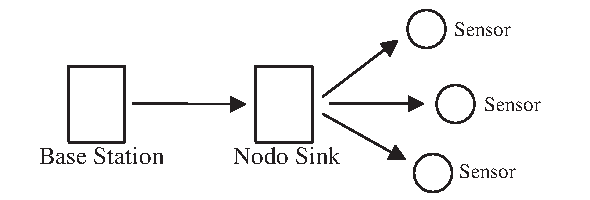
\includegraphics[scale=0.35]{img/exemplo.png}\\
    \caption{\it Exemplo de envio de comando}
\end{figure}




\chapter{CONCLUSÕES E TRABALHOS FUTUROS}
O sistema ainda se encontra longe de finalizado, porem a estrutura básica criada está solida é foi programada pensando principalmente em refatoramento e extensão.  Testes de unidade foram criados para garantir o continuo funcionamento 
das utilidades já implementadas e pretende-se criar um repositório para testes de regressão.\\

Este primeiro projeto orientado teve como objetivo criar a base do sistema. Portanto pretende-se no próximo trabalho, portar os \emph{softwares} cliente e servidores para o \emph{Android} e o \emph{Google App Engine}, implementar mais comandos, funcionalidades e integrar o sistema de rastreamento \emph{GPS}\footnote{Global Positioning System} com o \emph{Google Maps}


% ********** REFERÊNCIAS **********
%\bibliographystyle{abnt-alf}	 % Existem ainda: abbrv, acm, alpha, amsalpha, amsplain
\bibliographystyle{abnt-num}
\bibliography{bibliografia} % o nome do arquivo .bib com as referências
\include{bibliografia}															

%\apendice
\chapter{Linguagem gráfica do WebAPSEE}
\label{ApendiceA}

WebAPSEE-PML (\emph{Process Modeling Language}) é a linguagem gráfica usada para modelar processos no ambiente Open-WebAPSEE. Nesta linguagem, um modelo de processo pode ser construído a partir de símbolos gráficos conectados e o detalhamento do relacionamento com os outros componentes do modelo é feito através de formulários específicos que apóiam essa tarefa.


% \chapter{Entrada de Símbolos e Siglas}
% \par Para fazer a entrada de um símbolo, $\backslash$símbolo\{\simbolo{$\sigma$}{Descrição}\} \{Descriçao\} é a forma % correta. E, para definir uma sigla, $\backslash$sigla\{\sigla{ABNT}{Associação Brasileira de Normas Técnicas}\} % \{Descrição\} deve ser utilizado.
%  \par Obs.: Quando a sigla ou o símbolo aparecerem novamente no texto, não repita o comando, para que a sigla ou símbolo não se repita na lista correspondente.

% *********** APÊNDICES ***********
% ** Condicionados à necessidade **
% \apendice
% \chapter{Primeiro apêndice}
% \par Apêndices são textos elaborados pelo autor a fim de complementar sua argumentação.

% ************ ANEXOS *************
% ** Condicionados à necessidade **
% \anexo
% \chapter{Primeiro anexo}
% \par Anexos são documentos não elaborados pelo autor, que servem de fundamentação, comprovação ou ilustração.

\end{document}

% Quando o número de apêndices ou anexos vier a ser suficiente, é recomendado fazer um sumário separado para os apêndices, localizados imediatamente antes dos apêndices ou anexos. Nesse caso, no sumário principal, apenas é feito referência a este sumário específico.
